\documentclass[aspectratio=169]{beamer}

\usepackage[utf8]{inputenc}
\usepackage[spanish]{babel}
\usepackage{graphicx}
\usepackage{booktabs}
\usepackage{ragged2e}
\usepackage{minted}
\usepackage{xcolor}
\usepackage{tikz}
\usepackage{algorithm}
\usepackage{algorithmic}
\usepackage{minted}
\usepackage{listings}
\usepackage{tikz}
\usetikzlibrary{arrows.meta,positioning,fit,shapes.symbols}
\usetikzlibrary{arrows,shapes}
\definecolor{LightGray}{gray}{0.975}
\definecolor{links}{HTML}{2A1B81}
\hypersetup{colorlinks,linkcolor=,urlcolor=blue}
\AtBeginEnvironment{minted}{%
  \renewcommand{\fcolorbox}[4][]{#4}}

\usefonttheme{serif}

\usepackage{listings}
\lstdefinestyle{myCustomSQLStyle}{
  language=SQL,
  numbers=left,
  stepnumber=1,
  numbersep=10pt,
  tabsize=4,
  frame=single,
  backgroundcolor=\color{LightGray},
  breaklines=true,
  showspaces=false,
  showstringspaces=false
}

\newcommand\Wider[2][18mm]{%
    \makebox[\linewidth][c]{%
        \begin{minipage}{\dimexpr\textwidth+#1\relax}
            \raggedright#2
        \end{minipage}%
    }%
}

\title[Decision Trees]{Emergent Digital Technologies}
\subtitle{Decision Trees}
\author{et al}
\date{\today}

% Remove navigation symbols...
\setbeamertemplate{navigation symbols}{}

\defbeamertemplate*{footline}{shadow theme}{
    \leavevmode
    \hbox{
        \begin{beamercolorbox}[
                wd =        0.33\paperwidth,
                ht =        2.5ex,
                dp =        1.125ex,
                leftskip =  0.3cm plus1fil,
                rightskip = 0.3cm
            ]{author in head/foot}
            \flushleft EDT
        \end{beamercolorbox}
        \begin{beamercolorbox}[
                wd =        0.33\paperwidth,
                ht =        2.5ex,
                dp =        1.125ex,
                leftskip =  0.3cm plus1fil,
                rightskip = 0.3cm
            ]{author in head/foot}
            \insertshorttitle
        \end{beamercolorbox}
        \begin{beamercolorbox}[
                wd =        0.33\paperwidth,
                ht =        2.5ex,
                dp =        1.125ex,
                leftskip =  0.3cm plus1fil,
                rightskip = 0.3cm
            ]{title in head/foot}
            \hfill \insertframenumber\,/\,\inserttotalframenumber%
        \end{beamercolorbox}
    }
}

\AtBeginSection[]{
    \begin{frame}<beamer>
        \frametitle{Plan}
        \tableofcontents[currentsection]
    \end{frame}
}

\newcommand{\toRight}[1]{
    \begin{FlushRight}
        {\tiny #1}
    \end{FlushRight}
}

\begin{document}

\frame{\titlepage}

% \begin{frame}{EDT: Data Analytics.}
%     \centering
%     
\includegraphics[width=0.35\textwidth]{figures/book_cover}\\
%     \vspace{2mm}
%     {
%         \scriptsize
%         Content has been extracted from \textit{Database System Concepts 7ed (Chapter 11)}, by Abraham Silberschatz, Henry Korth \& S. Sudarshan, 2019.  Visit \url{https://db-book.com/}.
%     }
% \end{frame}

\section{Overview}

\begin{frame}{How to buy an avocado?}
    \Wider{
        \centering
        
\includegraphics[height=0.9\textheight]{figures/avocado}
    }
\end{frame}

\begin{frame}{How to buy an avocado...}
    \Wider{
        \centering
        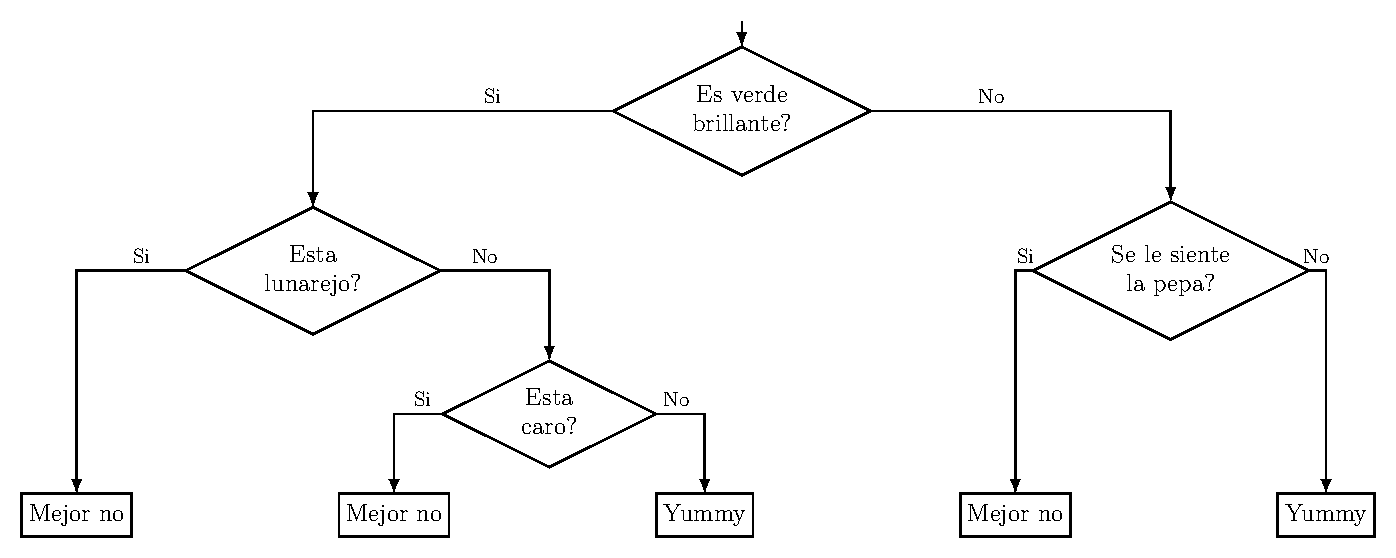
\includegraphics[width=\textwidth]{figures/buy_avocado}
    }
\end{frame}

\section{A simple recipe}

\begin{frame}{1. Measure the ``Mess'' (Entropy)}
    Before you start, look at your target (e.g., ``Should buy?'') and see how mixed the data is.
    \begin{itemize}
        \item \textbf{Entropy} measures the level of disorder or uncertainty.
        \item \textbf{Formula:} $H(S) = -\sum p_i \log_2(p_i)$
        \item \textbf{Maximum Mess:} If the data is $\frac{50}{50}$ ``Yes'' and ``No,'' your Entropy is \textbf{1.0}.
        \item \textbf{Perfectly Clean:} If the data is all ``Yes'' (or all ``No''), your Entropy is \textbf{0}.
    \end{itemize}
\end{frame}

\begin{frame}{2. Test Your ``Clues'' (Information Gain)}
    Pick a feature (like ``Color'' or ``Price'') and pretend to split the data by it.
    \begin{itemize}
        \item Calculate the entropy of the new groups you created.
        \item Subtract this from your original mess.
        \item The Result = \textbf{Information Gain (IG).}
        \item \textbf{Formula:} $IG(S, A) = H(S) - \sum \frac{|S_v|}{|S|} H(S_v)$
        \item It tells you how much ``cleaner'' the data became because of that clue.
    \end{itemize}
\end{frame}

\begin{frame}{3. Pick the Winner (The Root)}
    Compare the Information Gain of every feature. The one with the highest score becomes the node.
    \begin{itemize}
        \item \textbf{The Root Node:} This is your first and most important split.
        \item \textbf{Leaf Nodes:} If a branch becomes 100\% ``Yes'' or ``No,'' stop there!
        \item \textbf{Internal Nodes:} If a branch is still messy, you need to keep digging and find the next best clue.
    \end{itemize}
\end{frame}

\begin{frame}{4. Rinse and Repeat (Recursion)}
    For any branch that isn't a Leaf yet, repeat Steps 1--3 using only the data that traveled down that specific path.
    \vfill
    Repeat until:
    \begin{itemize}
        \item Every branch ends in a \textbf{Leaf} (0 Entropy).
        \item You \textbf{run out of features} to test.
        \item The tree reaches a \textbf{maximum depth} you've pre-set (to prevent it from getting too complex).
    \end{itemize}
\end{frame}

\begin{frame}{Pro-Tip: When to Stop?}
    In an informal setting, we usually stop when every leaf is ``pure''.
    \vspace{1cm}
    \begin{block}{Real-World Research}
    You often stop the tree early through \textbf{Pruning}. This prevents the model from ``memorizing'' the noise in the data (\textit{overfitting}\footnote{Have a loot at \href{https://tinyurl.com/46axxy39}{``What is overfitting?''} by IBM.}) rather than learning the actual underlying patterns.
    \end{block}
\end{frame}

\section{Foundation concepts}

\begin{frame}{What is Entropy?}
    \Wider{
        \centering
        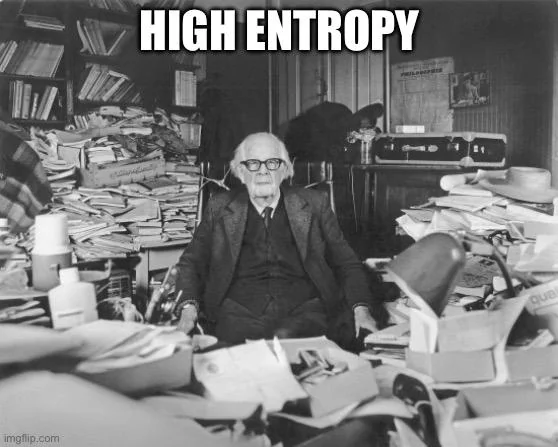
\includegraphics[height=0.8\textheight]{figures/entropy}
    }
\end{frame}

\begin{frame}{\text{ }}

    \Wider{
        \centering
        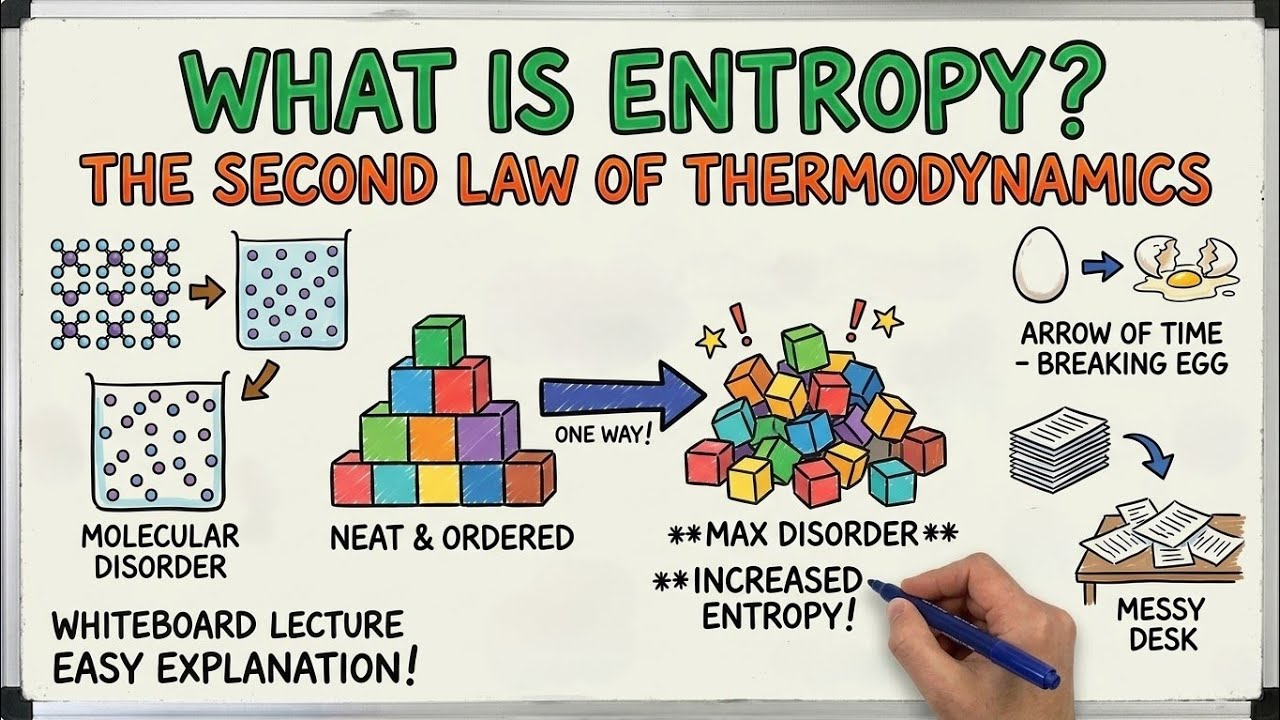
\includegraphics[width=0.8\textwidth]{figures/entropy2}
    }
    \toRight{\href{https://youtu.be/O7UX4S8zhk4?si=8hAzvdVVmMe_cfOP}{
What is Entropy? The Second Law of Thermodynamics Explained} by Afzaal Chemist}
\end{frame}

\begin{frame}{Understanding Entropy: The Measure of Disorder}
    \footnotesize
    \textbf{Entropy} $H(S)$ quantifies the uncertainty or impurity within a dataset $S$. In the context of Decision Trees, it determines how ``mixed'' our target classes are.

    \begin{block}{The Mathematical Formula}
        For a set with $c$ classes, entropy is defined as:
        \[ H(S) = \sum_{i=1}^{c} -p_i \log_2(p_i) \]
        Where $p_i$ is the proportion of samples belonging to class $i$.
    \end{block}

    \begin{itemize}
        \item \textbf{High Entropy (1.0):} Data is perfectly split (e.g., 50\% Yes, 50\% No). Uncertainty is at its maximum.
        \item \textbf{Low Entropy (0.0):} Data is perfectly ``pure'' (e.g., 100\% Yes). There is zero uncertainty.
        \item \textbf{Goal:} We use splits to move from high entropy at the root to low entropy at the leaves.
    \end{itemize}
\end{frame}

\begin{frame}{What is Information Gain?}
    \Wider{
        \centering
        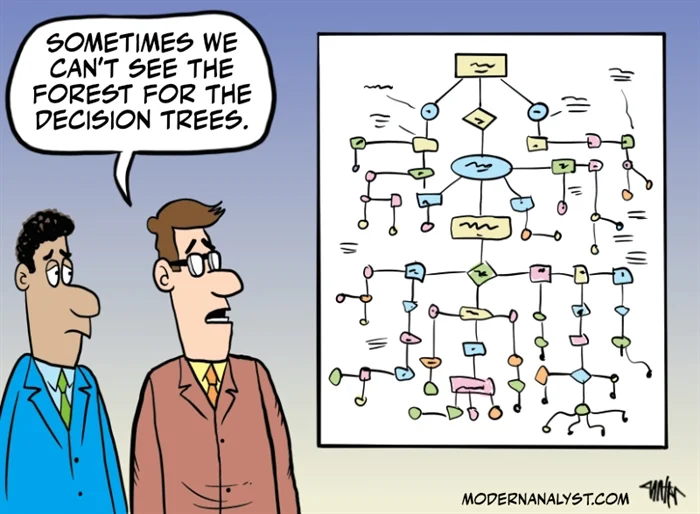
\includegraphics[height=0.8\textheight]{figures/ig}
    }
\end{frame}

\begin{frame}{\text{ }}

    \Wider{
        \centering
        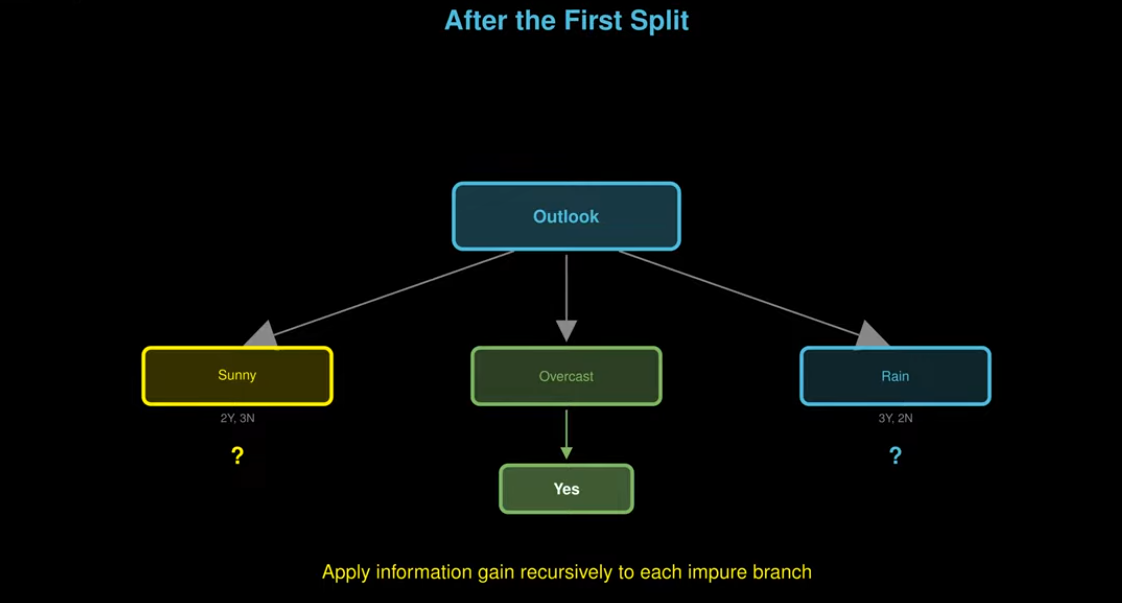
\includegraphics[width=0.8\textwidth]{figures/ig2}
    }
    \toRight{\href{https://youtu.be/tGcNOSgQFkI?si=QvJkdEaTiiMl45vJ}{Information Gain Explained | Module 2 Ep 3} by Nipun Batra}
\end{frame}

\begin{frame}{Information Gain: Choosing the Best Split}
    \footnotesize
    \textbf{Information Gain (IG)} measures the reduction in Entropy achieved by partitioning the data according to a specific attribute. It identifies which ``clue'' provides the most clarity.

    \begin{block}{The Mathematical Formula}
        The Information Gain for a set $S$ and attribute $A$ is:
        \[ IG(S, A) = H(S) - \sum_{v \in Values(A)} \frac{|S_v|}{|S|} H(S_v) \]
        Where:
        \begin{itemize}
            \item $H(S)$ is the Entropy before the split.
            \item $\frac{|S_v|}{|S|}$ is the weight of the subset $v$ resulting from the split.
            \item $H(S_v)$ is the Entropy of that subset.
            \item \textbf{The Selection Rule:} The attribute with the \textbf{highest} Information Gain is selected as the decision node.
            \item \textbf{Interpretation:} High IG means the attribute successfully organized the data into more homogeneous (pure) groups.
        \end{itemize}
    \end{block}
\end{frame}

\section{An example}

\begin{frame}{Introduction to the ``Play Tennis'' Dataset}
    The Play Tennis dataset is a classic example used to demonstrate the induction of Decision Trees via Entropy and Information Gain. It consists of 14 instances characterized by four environmental attributes.

    \begin{columns}
        \begin{column}{0.5\textwidth}
            \textbf{Target Variable:}
            \begin{itemize}
                \item \textbf{PlayTennis:} $\{Yes, No\}$
            \end{itemize}
            \vspace{0.5cm}
            \textbf{Predictor Attributes:}
            \begin{itemize}
                \item \textbf{Outlook:} $\{Sunny, Overcast, Rain\}$
                \item \textbf{Temperature:} $\{Hot, Mild, Cool\}$
                \item \textbf{Humidity:} $\{High, Normal\}$
                \item \textbf{Wind:} $\{Strong, Weak\}$
            \end{itemize}
        \end{column}

        \begin{column}{0.5\textwidth}
            \begin{block}{Dataset Characteristics}
                \begin{itemize}
                    \item \textbf{Total Samples:} 14
                    \item \textbf{Class Distribution:} 9 Yes / 5 No
                    \item \textbf{Goal:} Predict if conditions are suitable for playing tennis based on weather observations.
                \end{itemize}
            \end{block}
        \end{column}
    \end{columns}
\end{frame}

\begin{frame}{the ``Play Tennis'' Dataset}

    \Wider{
        \centering
        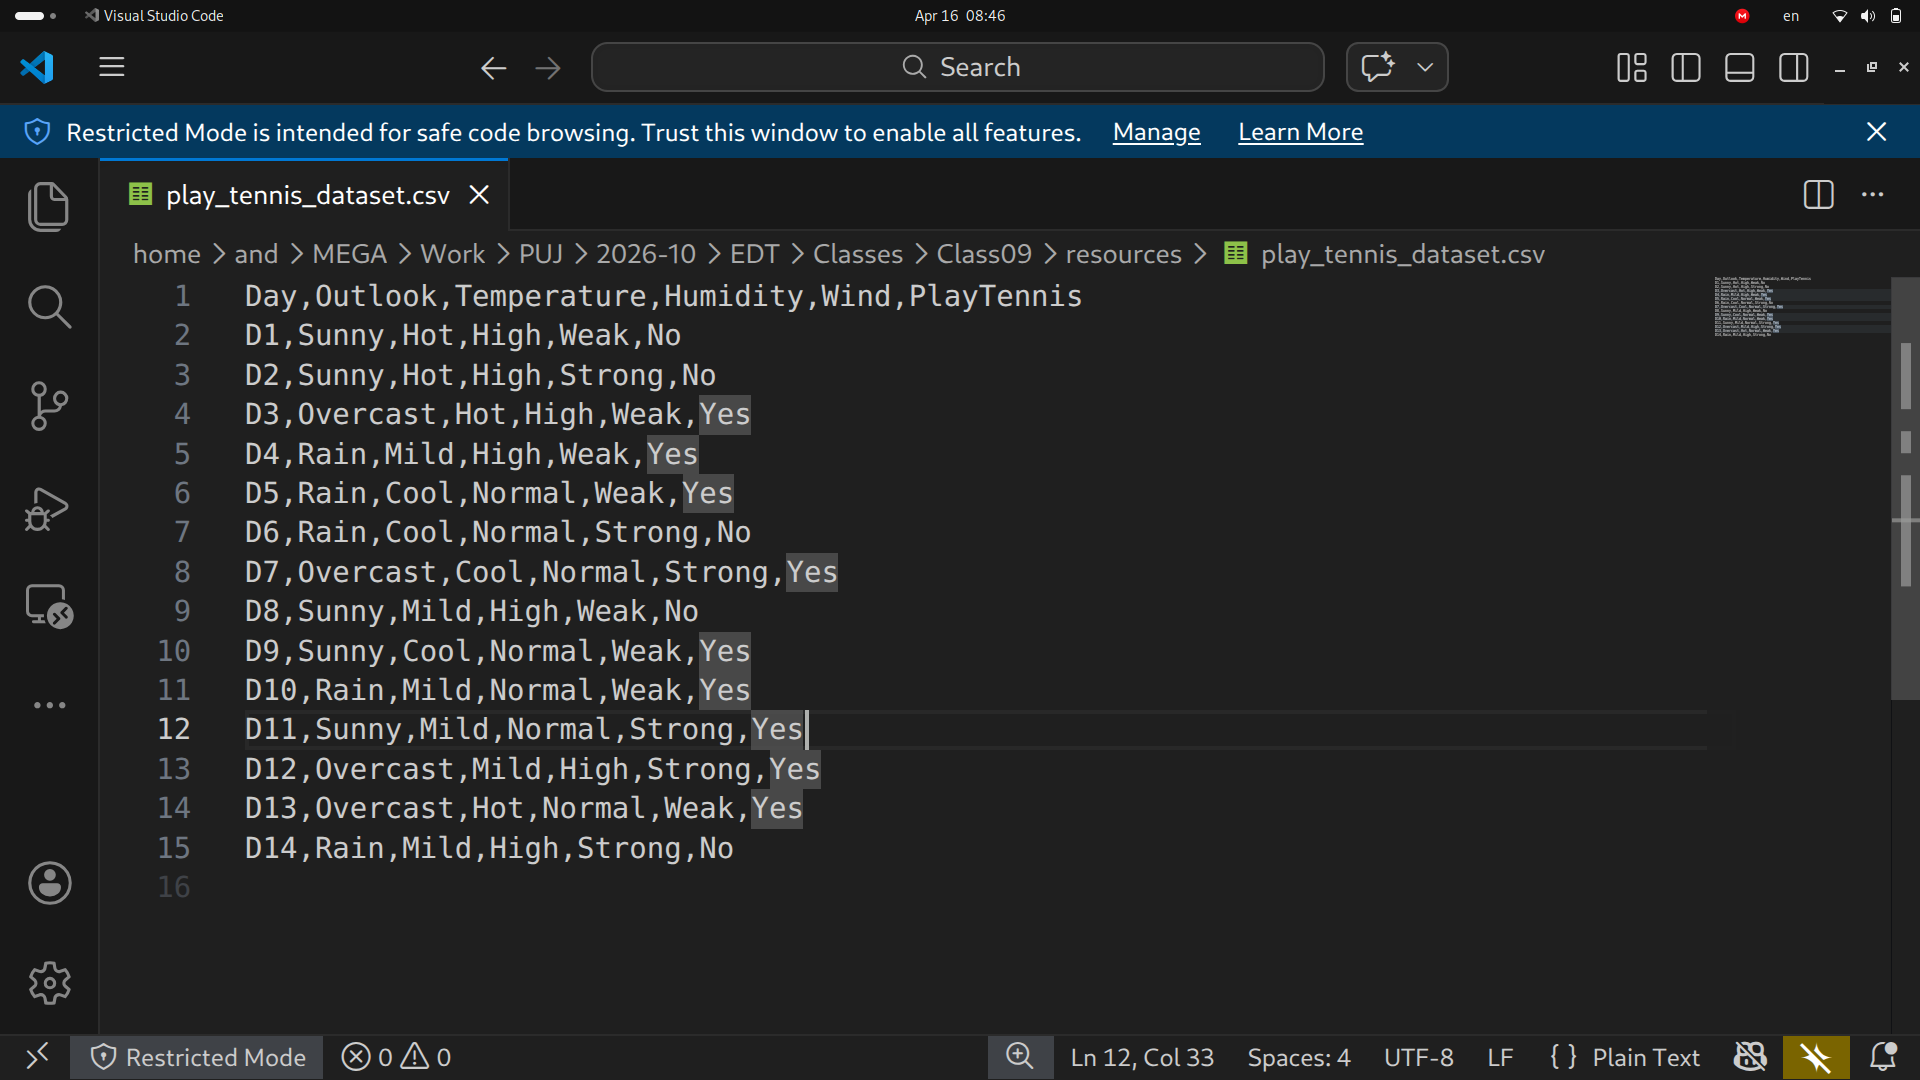
\includegraphics[width=0.8\textwidth]{figures/play}
    }
\end{frame}

% Total Entropy
\begin{frame}{Step 1: Calculating Total Entropy $H(S)$}
    Before splitting, we calculate the entropy of the entire dataset $S$.
    \[ H(S) = -\left(\frac{9}{14}\right) \log_2 \left(\frac{9}{14}\right) - \left(\frac{5}{14}\right) \log_2 \left(\frac{5}{14}\right) \]
    \vfill
    \begin{itemize}
        \item $P(Yes) = 9/14 \approx 0.643$
        \item $P(No) = 5/14 \approx 0.357$
        \item \textbf{Result:} $H(S) \approx 0.940$
    \end{itemize}
\end{frame}

% Evaluating Outlook
\begin{frame}{Step 2: Testing the First Attribute (Outlook)}
    We evaluate how much ``Outlook'' reduces the total entropy. Outlook has three values: Sunny, Overcast, and Rain.
    \begin{itemize}
        \item \textbf{Sunny:} (2 Yes, 3 No) $\rightarrow H \approx 0.971$
        \item \textbf{Overcast:} (4 Yes, 0 No) $\rightarrow H = 0$ (Perfectly Pure!)
        \item \textbf{Rain:} (3 Yes, 2 No) $\rightarrow H \approx 0.971$
    \end{itemize}
    \vfill
    Next, we calculate the weighted average of these entropies to find the ``remaining mess''.
\end{frame}

% IG for Outlook
\begin{frame}{Step 3: Information Gain for Outlook}
    Subtract the weighted entropy of the split from the original $H(S)$.
    \vfill
    \[ \text{Weighted Avg} = \left(\frac{5}{14} \times 0.971\right) + \left(\frac{4}{14} \times 0\right) + \left(\frac{5}{14} \times 0.971\right) \approx 0.693 \]
    \vfill
    \[ IG(S, \text{Outlook}) = 0.940 - 0.693 = \mathbf{0.247} \]
\end{frame}

\begin{frame}{Step 3: Information Gain for Humidity}
    \footnotesize
    To evaluate \textbf{Humidity}, we split the 14 samples ($9$ Yes, $5$ No) into \textbf{High} and \textbf{Normal} groups.
    Baseline Entropy $H(S) \approx 0.940$.

    \begin{itemize}
        \item \textbf{High Humidity:} 7 samples ($3$ Yes, $4$ No)
        \[ H(\text{High}) = -\frac{3}{7}\log_2\frac{3}{7} - \frac{4}{7}\log_2\frac{4}{7} \approx 0.985 \]
        \item \textbf{Normal Humidity:} 7 samples ($6$ Yes, $1$ No)
        \[ H(\text{Normal}) = -\frac{6}{7}\log_2\frac{6}{7} - \frac{1}{7}\log_2\frac{1}{7} \approx 0.592 \]
    \end{itemize}

    \begin{block}{Information Gain Calculation}
        \[ IG(S, \text{Hum}) = 0.940 - \left[ \frac{7}{14}(0.985) + \frac{7}{14}(0.592) \right] \]
        \[ IG(S, \text{Hum}) = 0.940 - 0.7885 = \mathbf{0.151} \]
    \end{block}
\end{frame}

\begin{frame}{Step 3: Information Gain for Wind}
    \footnotesize
    We evaluate the \textbf{Wind} attribute by splitting the 14 samples ($9$ Yes, $5$ No) into \textbf{Weak} and \textbf{Strong} groups.
    Baseline Entropy $H(S) \approx 0.940$.

    \begin{itemize}
        \item \textbf{Weak Wind:} 8 samples ($6$ Yes, $2$ No)
        \[ H(\text{Weak}) = -\frac{6}{8}\log_2\frac{6}{8} - \frac{2}{8}\log_2\frac{2}{8} \approx 0.811 \]
        \item \textbf{Strong Wind:} 6 samples ($3$ Yes, $3$ No)
        \[ H(\text{Strong}) = -\frac{3}{6}\log_2\frac{3}{6} - \frac{3}{6}\log_2\frac{3}{6} = 1.0 \]
    \end{itemize}

    \begin{block}{Information Gain Calculation}
        \[ IG(S, \text{Wind}) = 0.940 - \left[ \frac{8}{14}(0.811) + \frac{6}{14}(1.0) \right] \]
        \[ IG(S, \text{Wind}) = 0.940 - 0.892 = \mathbf{0.048} \]
    \end{block}
\end{frame}

\begin{frame}{Step 3: Information Gain for Temperature}
    \footnotesize
    We evaluate \textbf{Temperature} by splitting the 14 samples ($9$ Yes, $5$ No) into \textbf{Hot}, \textbf{Mild}, and \textbf{Cool} groups.
    Baseline Entropy $H(S) \approx 0.940$.

    \begin{itemize}
        \item \textbf{Hot:} 4 samples ($2$ Yes, $2$ No) $\rightarrow H = 1.0$
        \item \textbf{Mild:} 6 samples ($4$ Yes, $2$ No) $\rightarrow H \approx 0.918$
        \item \textbf{Cool:} 4 samples ($3$ Yes, $1$ No) $\rightarrow H \approx 0.811$
    \end{itemize}

    \begin{block}{Information Gain Calculation}

        \[ IG(S, \text{Temp}) = 0.940 - \left[ \frac{4}{14}(1.0) + \frac{6}{14}(0.918) + \frac{4}{14}(0.811) \right] \]
        \[ IG(S, \text{Temp}) = 0.940 - 0.911 = \mathbf{0.029} \]
    \end{block}
\end{frame}

% Root Selection
\begin{frame}{Step 4: Selecting the Root Node}
    We repeat the calculations for all other attributes:
    \begin{itemize}
        \item $IG(S, \text{Outlook}) = 0.247$
        \item $IG(S, \text{Humidity}) = 0.151$
        \item $IG(S, \text{Wind}) = 0.048$
        \item $IG(S, \text{Temperature}) = 0.029$
    \end{itemize}
    \begin{block}{Decision}
    \textbf{Outlook} has the highest Information Gain. It becomes our \textbf{Root Node}.
    \end{block}
\end{frame}

% Level 1 - The Sunny Branch
\begin{frame}{Step 5: Expanding the ``Sunny'' Branch}
    When Outlook is \textbf{Sunny}, the data is still mixed (2 Yes, 3 No). We must split again using only this subset.
    \vfill
    \textbf{Subset Features (Outlook = Sunny):}
    \begin{itemize}
        \item Humidity: (High $\rightarrow$ 3 No) and (Normal $\rightarrow$ 2 Yes)
        \item Wind: (Weak $\rightarrow$ 1 Yes, 2 No) and (Strong $\rightarrow$ 1 Yes, 1 No)
    \end{itemize}
\end{frame}

% IG for Humidity on Sunny Branch
\begin{frame}{Step 6: Final Split for the Sunny Branch}
    Evaluate Humidity on the ``Sunny'' subset ($H_{subset} = 0.971$).
    \begin{itemize}
        \item \textbf{High Humidity:} All 3 are ``No'' ($H = 0$).
        \item \textbf{Normal Humidity:} All 2 are ``Yes'' ($H = 0$).
    \end{itemize}
    \vfill
    \[ \text{Weighted Avg} = \left(\frac{3}{5} \times 0\right) + \left(\frac{2}{5} \times 0\right) = 0 \]
    \[ IG(\text{Sunny Subset}, \text{Humidity}) = 0.971 - 0 = \mathbf{0.971} \]
    \vfill
    Humidity provides a perfect split for the Sunny branch.
\end{frame}

% The Completed Tree
\begin{frame}{Step 8: Final Decision Tree Map}
    \begin{columns}[T]
        \begin{column}{0.45\textwidth}
            \textbf{Final Logic:}
            \begin{enumerate}
                \item \textbf{Root:} Outlook
                \item \textbf{If Overcast:} Leaf node $\rightarrow$ \textbf{Yes}.
                \item \textbf{If Sunny:} Split by \textbf{Humidity}.
                \begin{itemize}
                    \item High $\rightarrow$ \textbf{No}.
                    \item Normal $\rightarrow$ \textbf{Yes}.
                \end{itemize}
                \item \textbf{If Rain:} Split by \textbf{Wind}.
                \begin{itemize}
                    \item Weak $\rightarrow$ \textbf{Yes}.
                    \item Strong $\rightarrow$ \textbf{No}.
                \end{itemize}
            \end{enumerate}
        \end{column}
        \begin{column}{0.6\textwidth}
            \centering
            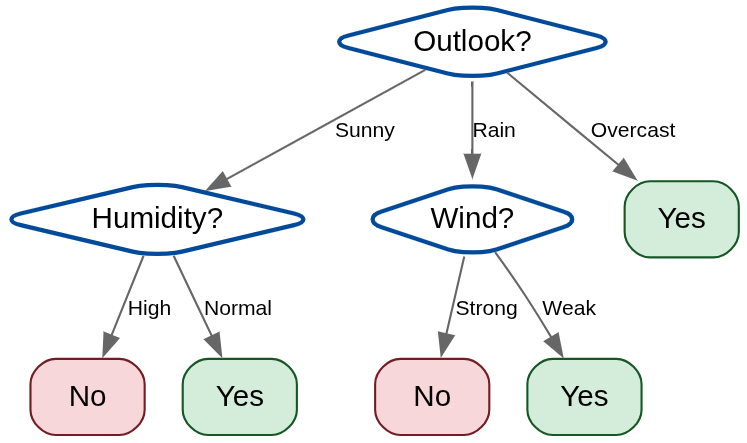
\includegraphics[width=1\textwidth]{figures/play_dt}
        \end{column}
    \end{columns}
\end{frame}

\begin{frame}{Takeaways: Decision Tree Induction}
    \small
    \begin{enumerate}
        \item \textbf{The Construction Recipe:} A systematic four-step process that uses Entropy and Information Gain to build tree structures through recursive splitting. \pause
        \item \textbf{Entropy as a Measure of Impurity:} A mathematical measure of uncertainty, ranging from a ``pure'' 0.0 to a ``maximum mess'' of 1.0, used to assess dataset disorder. \pause
        \item \textbf{Information Gain for Feature Selection:} The primary ``clue finder'' that identifies the best feature to split on by calculating the reduction in entropy achieved. \pause
        \item \textbf{Iterative Partitioning and Termination:} Tree growth continues recursively until branches reach zero-entropy ``leaf nodes'' or the model hits a pre-defined depth limit. \pause
        \item \textbf{Generalization through Pruning:} A critical technique that stops tree growth early to prevent ``overfitting,'' ensuring the model learns patterns rather than memorizing noise.
    \end{enumerate}
\end{frame}

% \begin{frame}{EDT: Data Analytics.}
%     \centering
%     
\includegraphics[width=0.35\textwidth]{figures/book_cover}\\
%     \vspace{2mm}
%     {
%         \scriptsize
%         Content has been extracted from \textit{Database System Concepts 7ed (Chapter 11)}, by Abraham Silberschatz, Henry Korth \& S. Sudarshan, 2019.  Visit \url{https://db-book.com/}.
%     }
% \end{frame}

\end{document}
